\section{Results}
\label{sec:results}

This section focuses on the evaluation and the results. First the evaluation of the recorded sensor data is shown. Subsequently the results are presented and discussed.


\subsection{Evaluation}
\label{subsec:evaluation}

The evaluation analyses the prediction occupancy and provides a measurement in order to depict the prediction performance. The evaluation in detail is depicted in the following.


\subsubsection{prediction approach}
\label{subsubsec:predictionApproach}

Alignment is a context time series prediction algorithm that is inspired by algorithms with a focus on computational biology and based on local alignment techniques like the Smith and Waterman algorithm (T.F. Smith and M.S. Waterman 1981). Basically Alignment compares two context sequences and therefore belongs to the branch of the pattern matching algorithms. For the use of number of passenger prediction, the first sequence represents the current sensed occupancy of the same location, called observation. The second sequence represents the history of passenger occupancy.
During the matching process that pattern in the history will be identified whose similarity to the given current observation pattern is the highest and therefore obtained the lowest penalty costs for a given cost matrix. Subsequently, the context that follows next to the identified pattern will be predicted. Figure~\ref{fig:alignmentApproach} illustrates the approach. In this example the values of five, nine and 17 are in the observation pattern as well as in the history pattern. Consequently both patterns match. The next value in the history pattern, the seven, is the prediction.

\begin{figure}[htb]
  \centering
  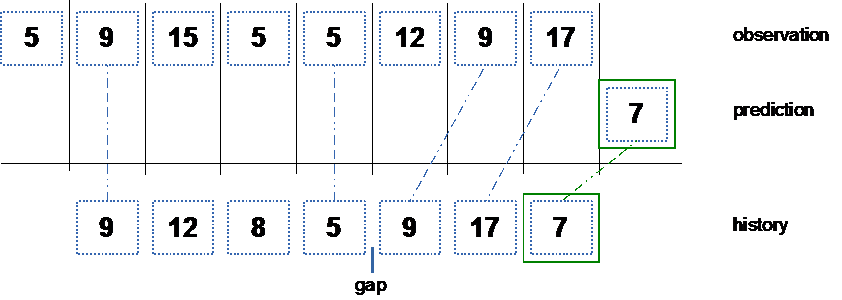
\includegraphics[width=0.9\linewidth]{alignmentApproach.png} 
  \caption{Alignment approach}
  \label{fig:alignmentApproach}
\end{figure}

If and how two pattern "match" is calculated during the matching process and noted in the cost matrix. Whenever to strings are not matching, e.g. because of a gap, a penalty is added. The goal is to stay with zero costs, the optimal value.

\begin{table}[htb]
  \center
  \begin{tabular}{|l|c|}
  \hline 
        & penalty \\ 
  \hline 
  match & 0 \\ 
  \hline 
  mismatch & 1 \\ 
  \hline 
  gap in first sequence & 1 \\ 
  \hline 
  gap in second pattern & 1 \\ 
  \hline 
  \end{tabular}
  \caption{example of alignment penalties}
  \label{tab:alignmentPenalties}
\end{table}

Penalty costs are a way to influence the alignment results. If gabs need to be avoided during the matching process, penalties can be increased. A different rating of gaps in the first and second sequence is possible. If gaps in the first sequence are not acceptable but gaps in the seconds sequence are tolerable penalty for gaps in the first sequence can be set higher than penalty for gaps in the second sequence. In general penalty cost can be freely selected. The highest similarity between history pattern and the current observation is given on the lowest penalty costs. Figure 3 depicts the filled cost matrix.


\subsubsection{Performance measurement}
\label{subsubsec:performanceMeasurement}

In order to understand how good the predicted value and the actual value match, a performance measurement is needed. A standard measurement is the accuracy. The accuracy describes the performance of the system in a percent value. An accuracy value of 100~\% represents a perfect prediction, while 0~\% represents a poor prediction. In case of the Usermodel an easy way of calculation could be, a division of the lower number of passenger by the higher number of passenger value as depicted in equation~\ref{eq:accuracy}.

\begin{equation}
accuracy = \frac{lower~value}{heigher~value}
\label{eq:accuracy}
\end{equation}

Following this equation the accuracy for a predicted value of two and an actual value of one is calculated to 50~\% (equation~\ref{eq:accuracyExample}).

\begin{equation}
accuracy = \frac{1}{2} = 0.5 = 50~\%
\label{eq:accuracyExample}
\end{equation}

In this example the accuracy is 50~\% even though the predicted value is close to the actual value. Predicted and actual value differs only by one. A difference of one person does not have big impact on the controller in order to satisfy the restrictions. Therefore the accuracy does not fulfil the needs as a performance measure.

Instead the absolute difference between the predicted number of passenger as well as the actual number of passenger seems to provide a meaningful measurement. A measurement-value of zero~(0) represents a perfect prediction, while the higher the worse the prediction. In this deliverable absolute difference between predicted number of passenger and the actual number of passenger is used as the performance measure for the detection accuracy of the number of passenger prediction.
Staying in the mentioned example the accuracy is calculated to one (Equation~\ref{eq:diffExample}).

\begin{equation}
accuracy = |1-2| = 1
\label{eq:diffExample}
\end{equation}

A difference between predicted and actual number of passenger of one allows the conclusion of a good prediction. 


\subsection{Results}
\label{subsec:results}

This section depicts the prediction results and is aimed to figure out:

\begin{enumerate}
  \item the overall prediction accuracy,
  \item the best performing penalty setup,
  \item the best performing history and observation length, and
  \item the average prediction duration.
\end{enumerate}
